
\chapter{Computation of the Solution of the Approximate
  Problem}\label{chap4} 

\section{Introduction}\label{chap4:ssec4.1} 

THE\pageoriginale SOLUTION OF THE APPROXIMATE PROBLEM. Find $u_h\varepsilon
V_h$ such that 

\setcounter{equation}{0}
\begin{equation}\label{chap4:eq4.1}
a(u_h, v_h)=L(v_h) \; \forall v_h\varepsilon V_h,
\end{equation}
can be found using either iterative methods or direct methods. We
describe these methods in this chapter.

Let $\{w_i\}_{1\leq i\leq N(h)}$ be a basis of $V_h$. Let $A=(a(w_i,
w_j))$ and $b=(L(w_i))$. If $a(\cdotp,\cdotp)$ is symmetric, then
\eqref{chap4:eq4.1} is equivalent to the minimization problem 
\begin{equation}\label{chap4:eq4.2}
J(u_h)=\min\limits_{v_h\varepsilon V_h}\; J(v_h),
\end{equation}
where $J(v)=\frac{1}{2}v^TAv-v^Tb,\;
v\varepsilon\mathbb{R}^{N(h)}$. Here we identify $V_h$ and
$\mathbb{R}^{N(h)}$ through the basis $\{w_i\}$ and the natural basis
$\{e_i\}$ of $\mathbb{R}^{N(h)}$. $u_h$ is a solution of
\eqref{chap4:eq4.2} $\Iff Au_h=b$. Iterative methods are applicable
only when $a(\cdotp,\cdotp)$ is symmetric.

\section{Steepest Descent Method}\label{chap4:ssec4.2}
Let $J:\mathbb{R}^N\to\mathbb{R}$ be differentiable.

In the steepest descent method, at each iteration we move along the
direction of the negative gradient to a point such that the functional
value of $J$ is reduced. That is, let
$x^\bullet\varepsilon\mathbb{R}^N$ be given. Knowing $x^n\varepsilon
\mathbb{R}^N$, we define $x^{n+1}\varepsilon\mathbb{R}^N$ by 
\begin{equation}\label{chap4:eq4.3}
x^{n+1}=x^n-\lambda^n\; J'(x^n),
\end{equation}
where $\lambda^n$ minimizes the functional 
\begin{equation}\label{chap4:eq4.4}
\phi(\lambda)=J\left(x^n-\lambda J'(x^n)\right)
\end{equation}\pageoriginale

In the case
$$
J(x)=1/2\; x^T Ax-x^Tb,
$$
$\lambda^n$ can be computed explicitly. It is easy to see that 
$$
J'(x)=Ax-b.
$$
Since $\lambda^n$ minimizes $\phi(\lambda)$, we have 
\begin{equation}\label{chap4:eq4.5}
\phi'(\lambda^n)=\left(J'(x^n-\lambda^n J'(x^n)), -J'(x^n)\right)=0
\end{equation}
Let
$$
r^n=J'(x^n)=Ax^n-b.
$$
Then \eqref{chap4:eq4.5} implies
\begin{equation}\label{chap4:eq4.6}
\lambda^n=\frac{(r^n,\; r^n)}{(Ar^n, r^n)}.
\end{equation}
For proving an optimal error estimate for this scheme we need
Kantorovich's inequality which is left as an exercise.

\setcounter{exercise}{0}
\begin{exercise}\label{chap4:exr1}
(See LUENBERGER \cite{key30}).

Prove the Kantorovich's inequality 
\begin{equation}\label{chap4:eq4.7}
\frac{(Ax, x)\;(A^{-1}x, x)}{\parallel x\parallel^4}\leq
\frac{(M+m)^2}{4mM}
\end{equation}
where $A$ is symmetric, positive definite matrix with 
$$
m=\underset{x\neq 0}{\Inf}\frac{(Ax,x)}{\parallel x\parallel^2}>0, M=
\underset{x\neq 0}{\Sup}\frac{(Ax, x)}{\parallel x\parallel^2}
$$
\end{exercise}

\setcounter{THM}{0}
\begin{THM}\label{chap4:THM1}
For any $x_\circ \varepsilon X$ the sequence $\{x_n\}$ defined by 
$$
x_{n+1}=x_n+\frac{(r_n,r_n)}{(r_n, Ar_n)}r_n,
$$\pageoriginale
where
$$
r_n=b-Ax_n,
$$
converges to the unique solution $\overline{x}$ of
$Ax=b$. Furthermore, defining
$$
E(x)=((x-\overline{x}), A(x-\overline{x})) 
$$
we have the estimate
$$
\parallel x_n-\overline{x}\parallel^2\leq\frac{1}{m} E(x_n)\leq
\frac{1}{m}\left(\frac{M-m}{M+m}\right)^{2n}E(x_\circ).
$$
\end{THM}

\begin{proof}
We have 
\begin{align*}
E(x) &= (x-\overline{x}, A(x-\overline{x}))\\
&= 2J(x)+(\overline{x},\;A\overline{x}),\\
\intertext{where} 
J(x) &= 1/2 (x, Ax)-(b, x).
\end{align*}

It is easy to see that 
$$
\dfrac{E(x_n)-E(x_{n+1})}{E(x_n)}=\dfrac{(r_n, r_n)^2}{(r_n, Ar_n)(r_n,
A^{-1}r_n)}\geq\dfrac{4Mm}{(M+m)^2}
$$
by Kantorovich inequality. Therefore
$$
\dfrac{E(x_{n+1})}{E(x_n)}\leq\left(\dfrac{M-m}{M+m}\right)^2.
$$
This implies 
$$
E(x_{n+1})\leq\left(\dfrac{M-m}{M+m}\right)^{2(n+1)}E(x_\circ).
$$

From\pageoriginale the definition of $m$ we obtain
$$
\parallel x_n-\overline{x}\parallel^2\leq\frac{1}{m}E(x_n)\leq\frac{1}
{m}\left(\frac{M-m}{M+m}\right)^{2.n}E(x_\circ).
$$

The condition number of $A$ is defined by $\cond (A)=\frac{M}{m}$. We
have 
$$
\left(\frac{M-m}{M+m}\right)^2\sim 1-\frac{2m}{M}=1- \frac{2}
{\cond (A)}
$$

If the condition number of $A$ is smaller, then the convergence is
faster. The steepest descent method is not a very good method for
finite elements, since $\cond (A)\sim C/h^2$ when $V_h\subset
H^1(\Omega)$. 
\end{proof}

\section{Conjugate Gradient method}\label{chap4:ssec4.3}
\begin{def*}\label{chap4:def}
The directions $w_1, w_2\varepsilon\mathbb{R}^N$ are said to be
\emph{conjugate} with respect to the matrix $A$ if $w_1^T\;A\;w_2=0$. 

In the conjugate gradient method, we construct conjugate directions
using the gradient of the functional. Then the functional is minimized
by proceeding along the conjugate direction. We have 
\end{def*}

\begin{THM}\label{chap4:THM2}
Let $w^1, w^2,\ldots,w^N$ be $N$ mutually conjugate directions. Let
$$
x^{k+1}=x^k-\lambda^k w^k
$$
where $\lambda^k$ minimizes
$$
\phi(\lambda)=J(x^k-\lambda w^k), \; \lambda\varepsilon\mathbb{R}.
$$
When\pageoriginale $x^1\varepsilon \mathbb{R}^N$ is given, we have 
$$
x^{N+1}=x^*
$$
where
$$
Ax^*=b.
$$
\end{THM}

\begin{proof}
Let 
$$
r^n=-J'(x^n)=b-Ax^n.
$$
Since $\lambda^k$ minimizes $\phi(\lambda)$ we have 
$$
\phi(\lambda^k)=(J'(x^k-\lambda^kw^k),-w^k)=0.
$$
This gives
\begin{equation}\label{chap4:eq4.8}
\lambda^k=\frac{(r^k)^Tw^k}{(w^k)^TAw^k}
\end{equation}

Since $w^1, w^2,\ldots,w^N$ are mutually conjugate directions, they
are linearly independent. Therefore there exist $\alpha_i, 1\leq i\leq
N$, such that 
$$
x^1-x^*=\sum\limits_{k=1}^N\alpha_k\; w^k.
$$

From this, using the fact that $w^j$ are mutually conjugate, we obtain
$$
(x^1-x^*)^T Aw^j=\alpha_j(w^j)^TAw^j.
$$
This gives 
\begin{equation}\label{chap4:eq4.9}
\alpha_j=\frac{(x^1-x^*)^T\;Aw^j}{(w^j)^T\;Aw^j}.
\end{equation}
Using\pageoriginale induction we show that 
$$
\alpha_k=\lambda^k.
$$
Since $Ax^*=b$, we have 
$$
r^1=Ax^1-b=A(x^1-x^*).
$$
This shows that
$$
\alpha_1=\lambda^1.
$$

Let $\alpha_i=\lambda^i$ for $1\leq i\leq k-1$.

\noindent From the definition of $x^k$ we obtain
$$
x^k=x^1-\sum\limits_{i=1}^{k-1}\lambda^iw^i=x^1-\sum\limits_{i=1}^{k-1}
\alpha_i \;w^i,
$$
(by induction hypothesis). Since 
$$
(w^i)^T\;Aw^k=0\quad\text{for}\quad 1\leq i\leq k-1,
$$
we get
$$
(x^k-x^1)^T\; Aw^k=0
$$
This together with \eqref{chap4:eq4.8} and \eqref{chap4:eq4.9} shows
that 
$$
\alpha_k=\lambda^k
$$
Thus $\alpha_k=\lambda^k$ for $1\leq k\leq N$.

The definition of $x^k$ implies
$$
x^{N+1}=x^1-\sum\limits_{i=1}^N\lambda^i \;w^i=x^1-
\sum\limits_{i=1}^N\alpha_iw^i=x^*
$$
\end{proof}

\subsubsection{\bf Algorithm for Conjugate Gradient Method}

\begin{THM}\label{chap4:THM3}
Let $x_\circ\varepsilon\mathbb{R}^N$. Define $w^1=b-Ax^1$. Knowing
$x^n$ and\pageoriginale $w^{n-1}$ we define $x^{n+1}$ and $w^n$ by 
\begin{align*}
x^{n+1}&= x^n+\alpha_nw^n\\
w^n &= r^n+\beta_nw^{n-1},
\end{align*}
where
$$
r^n=b-Ax^n, \alpha_n=\frac{(r^n,w^n)}{(w^n,Aw^n)},\beta_n=
\frac{(r^n,r^n)}{(r^{n-1},r^{n-1})}
$$

Then $w^n$ are mutually conjugate directions and $x^{N+1}$ is the
unique solution of $Ax=b$. 
\end{THM}

A proof of this theorem can be found in LUENBERGER \cite{key31}. It can be
shown that 
$$
x^n-x^{N+1}\sim \left(\frac{1-\sqrt{c}}{1+\sqrt{c}}\right)^n,
$$
where $c=m/M$. Thus the convergence rate in the conjugate gradient
method is faster than in the steepest descent method, at least for
quadratic functionals.

\section{Computer Representation of a Triangulation}\label{chap4:ssec4.4} 
\begin{figure}[H]
\centering
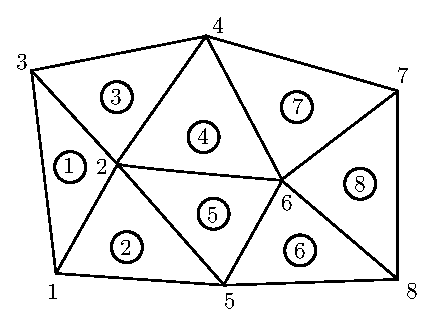
\includegraphics{figure/fig4.1.eps}
\caption{}\label{fig4.1}
\end{figure}


Let\pageoriginale $T_h$ be a triangulation of the domain $\Omega$. We
number the nodes of the triangulation and the triangles in $T_h$. Let
\begin{align*}
NS &= \#\quad\text{of nodes of}\quad T_h,\\
NT &= \#\quad\text{of triangles in}\quad T_h.
\end{align*}
The triangulation is uniquely determined by the two matrices
$$
Q(2,\; NS)=(q_{ij})\quad\text{and}\quad ME(3,\; NS)=(m_{jk}),
$$
where $q_{ij}$ denotes the $i^{th}$ coordinate of the $j^{th}$ node
and $m_{jk}$ denotes the $j^{th}$ vertex of the $k^{th}$ triangle.

The matrix $ME$, corresponding to the triangulation in the above
figure is 
\begin{equation*}
ME=
\begin{pmatrix}
1&1&2&2&2&6&4&6\\
2&5&4&6&5&5&6&8\\
3&2&3&4&6&8&7&7
\end{pmatrix}
\end{equation*}

In some problems it is better to know the boundary nodes. The array
$NG(NS)$ defined by 
\begin{equation*}
NG(i)=
\begin{cases}
1\quad\text{if}\quad i\varepsilon\Gamma\\
0\quad\text{otherwise}
\end{cases}
\end{equation*}
is used for picking boundary nodes.

\begin{exercise}\label{chap4:exr2}
Draw the triangulation
\begin{equation*}
Q=
\begin{pmatrix}
0&1&1&0&0.5&0.5&0.5&1&0\\
0&0&1&1&0.5&1&0&0&0.5
\end{pmatrix}
\end{equation*}
\begin{equation*}
ME=
\begin{pmatrix}
2&2&6&3&4&4&1&5\\
7&5&5&6&6&9&7&7\\
5&8&8&8&9&5&9&9
\end{pmatrix}
\end{equation*}\pageoriginale
\end{exercise}

\section{Computation of the Gradient.}\label{chap4:ssec4.5}
In the Neumann problem we have 
$$
(J'(u),\; v)=\int\limits_\Omega(\nabla u.\nabla v+a_\circ uv)-
\int\limits_\Omega \;fv.
$$
We now give a practical way of computing the gradient $J'(u)$.

Let $w_i$ be the basis function in $V_h$ which takes the value $1$ at
the $i^{th}$ node and zero at the other nodes. Let $V_h$ be defined by
$\mathbb{P}_1$ Lagrange finite element. Let
$$
u=(u_i)_{1\leq i\leq NS}
$$
be given. We want to compute $J'(u)$. Let $(J'(u)_i=(J'(u);w_i)$ and 
$$
B_i=\int\limits_\Omega\nabla u.w_i\,dx= \sum\limits_{K\varepsilon T_h}
\int\limits_K\nabla u.\nabla w_i\,dx.
$$
We know that 
\begin{equation*}
w_i=
\begin{cases}
\lambda_j^k\quad\text{if}\quad i=m_{jk},\quad\text{for some}\quad j
\quad\text{and}\quad k\\
0\quad\text{otherwise},
\end{cases}
\end{equation*}
where $\lambda_j^k$ is the $j^{th}$ rycentric coordinate of the
$k^{th}$ triangle. Therefore
\begin{align*}
B_i &= \sum\limits_{1\leq j\leq 3, 1\leq k\leq NT, i=m_{jk}}a_j^k,\\
a_j^k &= \int\limits_{K_k}\nabla u.\nabla\lambda_j^k\,dx,
\quad\text{where}\quad K_k
\end{align*}
is\pageoriginale the triangle corresponding to the $k^{th}$ element.

\subsubsection{\bf Algorithm to Compute B.}

\hspace{.5cm} Set $\quad B=0$

for $\quad k=1, 2,\ldots, NT$;

for $\quad j=1, 2, 3$,

do $\quad B_{m_{jk}}=B_{m_{jk}}+a_j^k$.

\subsubsection{\bf Computation of the ${a_j^k}{}_{'}s$.} Since
$u=(u_i)_{1\leq i\leq NS}$ and we take $\mathbb{P}_1$ Lagrange finite
elements, we have 

\begin{align*}
u &= \sum\limits_{j=1}^3\lambda_j^k u_{m_{jk}}\quad\text{in}\quad
K_k,\\
&= ax+by+c,\quad\text{say}.
\end{align*}
Let $(\xi_i,\eta_i), 1\leq i\leq 3$, be the coordinates of the
vertices of $K_k$. Let $w_j=u_{m_{jk}}$. Then $a, b$ are found from
the equations
\begin{equation}
\begin{split}\label{chap4:eq4.10}
a\xi_1 + b\eta_1 + c &= w_1,\\
a\xi_2 + b\eta_2 + c &= w_2,\\
a\xi_3 + b\eta_3 + c &= w_3,
\end{split}
\end{equation}
as 
\begin{align} 
a &=
\frac{(w_1-w_3)(\eta_2-\eta_3)-(w_2-w_3)(\eta_1-\eta_3)}{C_2}\label{chap4:eq4.11}
\\
b &= -\frac{(w_1-w_3)(\xi_2-\xi_3)-(w_2-w_3)(\xi_1-\xi_3)}{C_2}\label{chap4:eq4.12}
\end{align}
where
$$
C_2=(\xi_1-\xi_3)(\eta_2-\eta_3)-(\xi_1-\xi_2)(\eta_1-\eta_3).
$$
Hence\pageoriginale $\nabla u=\binom{a}{b}$ is determined. 

If $\lambda_j^k=a^jx+b^jy+c$, then $a^j$ and $b^j$ are got from
\eqref{chap4:eq4.11} and \eqref{chap4:eq4.12} by taking
$w_i=\delta_{ij}$. Note that $C_2=1/2$ area $K_k$. Then
$a_j^k=C_2/2\;(aa_j+bb_j)$. 

\section{Solution by Direct Methods}\label{chap4:ssec4.6} 
In Section \ref{chap4:sec2} and \ref{chap4:sec3} we gave algorithms to
solve the equation $Ax=b$ when $A$ is symmetric and positive
definite. When $A$ is not symmetric or $A$ is sparse, direct methods
can be used to solve the equation $Ax=b$.

\subsection{Review of the Properties of Gaussian
  Elimination} \label{chap4:sec1}
 The principle of Gaussian elimination is to decompose $A$ into a product $LU$ where $L$ is lower triangular and $U$ is upper triangular so that the linear system 
$$ 
Ax=b
$$
is reduced to solving 2 linear systems with triangular matrices 
\begin{align*}
Ly &= b,\\
Ux &= y.
\end{align*}
Each of these is very easy to solve. For $Ly=b, y=(y_i),y_1$ is given
by the first equation, hence $y_2$ is given by the second since $y_1$
is already known, etc.

To decompose $A$ into $LU$, one proceeds iteratively. Let 
$$
A^{(k)}=\left(a_{ij}^{(k)}\right)1\leq i, j\leq N\quad\text{'}
$$
be\pageoriginale such that 
$$
a_{ij}^{(k)}=0\quad\text{for}\quad 1\leq j\leq k-1\quad\text{and}\quad
i>j.
$$
\begin{figure}[H]
\centering
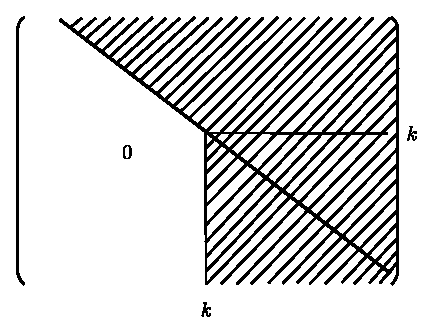
\includegraphics{figure/fig4.2.eps}
\caption{}\label{fig4.2}
\end{figure}

Then $U$ is $A^{(N)}$. 

To get $A^{(k+1)}$ from $A^{(k)}$ one adds the $k^{th}$ equation
multiplied by a scaling factor of the $i^{th}$ equation in order to
have $a_{ik}^{(k+1)}=0$. The scaling factor has to be 
\begin{equation}\label{chap4:eq4.13}
\begin{split}
-\frac{a_{ik}^{(k)}}{a_{kk}^{(k)}},\quad\text{and hence}\\
a_{ij}^{(k+1)}=a_{ij}^{(k)}-\frac{a_{ik}^{(k)}\;a_{kj}^{(k)}}
{a_{kk}^{(k)}} i,\quad j=k+1,\ldots,n.
\end{split}
\end{equation}

For a full matrix the order of operations for this process is
$N^3/3$. For a band matrix, \ie a matrix such that 
$$
a_{ij}=0\quad\text{if}\quad |i-j|\geq w,
$$
We see that if $|i-j|\geq w$, then either $|k-i|$ or $|k-j|$ is
greater than $w+1$, provided that $i, j\geq k+1$. Hence in the formula
\eqref{chap4:eq4.13} an element which is outside the band is never
modified since the corrective term in \eqref{chap4:eq4.13} is a
always zero. 
\begin{figure}[H]
\centering
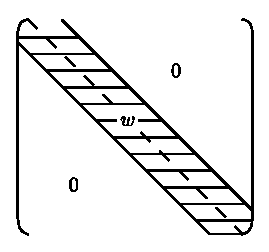
\includegraphics{figure/fig4.3.eps}
\caption{}\label{fig4.3}
\end{figure}

More\pageoriginale precisely we have

\setcounter{propn}{3}
\begin{propn}\label{chap4:propn4}
For a band matrix $A$ with bandwidth $w$, at the $k^{th}$ step of the
Gaussian elimination, only $w^2$ ``corrective elements'' have to be
computed and added to the submatrix.
\begin{equation*}
\begin{pmatrix}
a_{k+1, k+1} & \cdots & a_{k+1, k+w}\\
\vdots \\
a_{k+w, k+1} & \cdots & a_{k+w, k+w}
\end{pmatrix}
\end{equation*}
Note that we get an evaluation of the number of operations for the
process which is about $Nw^2$ (instead of $N^3/3$).
\end{propn}

\subsection{Stiffness Matrix and Stiffness Submatrix}\label{chap4:sec2} 
For simplicity we consider the Neumann problem. Find $u_h\varepsilon
V_h$ such that 
$$
a(u_h, v)=L(v)\forall\; v\varepsilon V_h,
$$
where $V_h$ is a finite dimensional subspace of $H^1(\Omega)$
constituted with functions which are continuous and piecewise linear
on the elements of the triangulation $T_h$ and 
$$
a(u, v)=\int\limits_\Omega(\nabla u.\nabla v+uv)\,dx.
$$\pageoriginale
For $(w_i)_{1\leq i\leq N}$, a basis of $V_h$ (where $N$ denotes the
number of vertices of $T_h$), we have 
$$
a(u, v)=\sum\limits_{i, j=1}^N u_ia_{ij}v_j,
$$
where $v_i$ (respectively $u_i$) denote the value of $v$ (respectively
$u$) at the $i^{th}$ vertex of $T_h$ and
$$
a_{ij}=\int\limits_\Omega (\nabla w_i\; \nabla w_j+w_iw_j)\,dx.
$$

But this is not a practical way to compute the elements $a_{ij}$ of
the matrix $A$ of the linear system to be solved, since the support of
the $w_i$ involves several elements of $T_h$. Instead one writes
$$
a(u, v)=\sum\limits_{K\varepsilon T_h}\int\limits_K(\nabla u.\nabla
v+uv)\,dx.
$$
Hence, as 
\begin{align*}
u(x) &= \sum\limits_{\alpha =1}^3 u_{m_{\alpha
K}}\lambda_\alpha^K(x),\\
v(x) &= \sum\limits_{\beta =1}^3v_{m_{\beta K}}\lambda_\beta^K(x),
\end{align*}
in the element $K$, where $(m_{\alpha K})_{\alpha =1, 2, 3}$ denotes
the 3 vertices of the element $K$ and $\lambda_\alpha^K(x)$ the
associated barycentric coordinates. One has 
$$
\sum\limits_{i, j=1}^Nu_ia_{ij}v_j=\sum\limits_{K\varepsilon T_h}
\sum\limits_{\alpha,\beta =1}^3u_{m_{\alpha K}}v_{m_{\beta K}}
a_{\alpha\beta}^K, 
$$\pageoriginale
where
$$
a_{\alpha\beta}^K=\int\limits_K(\nabla\lambda_\alpha^K.\nabla\lambda_\beta^K
+\lambda_\alpha^K\lambda_\beta^K)\,dx.
$$
The matrix $A^K=(a_{\alpha\beta}^K)_{1\leq\alpha,\beta\leq 3}$ is
called the \emph{element stiffness matrix} of $K$.

A convenient algorithm to compute $A$ is then the following
\emph{Assembling algorithm}.
\begin{equation*} 
\begin{cases}
1.\quad\text{Set}\quad A=0\\
2.\quad\text{For}\quad K\varepsilon T_h,\quad\text{compute $A^K$
and for $\alpha,\beta=1, 2, 3$ make}\\
\quad a_{m_{\alpha K},m_{\beta 
K}}= a_{m_{\alpha K},m_{\beta K}}+a_{\alpha\beta}^K.
\end{cases}
\end{equation*}

\begin{exercise}\label{chap4:exr3}
Write a Fortran subroutine performing the assembling algorithm
(without the computation of the element stiffness matrices $A^K$ which
will be assumed to be computed in another subroutine).
\end{exercise}

\subsection{Computation of Element Stiffness Matrices} \label{chap4:sec3}
We shall consider more sophisticated 
elements, \eg\ the triangular, qua\-dra\-tic element with 6 nodes.

The midside points have to be included in the numbering of the
vertices to describe properly the triangulation. For each element $K$,
one has to give the 6 numbers of its 6 nodes in the global numbering, 
$$
m_{\alpha K},\alpha =1,\ldots, 6.
$$\pageoriginale

The assembling algorithm of last section is still valid except that
$\alpha$ and $\beta$ range now from $1$ to $6$ and that
$\lambda_\alpha^K$ has to be replaced by $p_\alpha^K,\alpha
=1,2,\ldots,6$, the local basis functions of the interpolation (see
chapter \ref{chap3}).

To compute the element stiffness matrix
$$
A^K=\left(a_{\alpha\beta}^K\right)_{\alpha,\beta=1,\ldots,6},
$$
one introduces the mapping,
$$
F:\hat{K}\to K
$$
where $\hat{K}$ is the triangle $(0, 0), (1, 0), (0, 1)$. Since $F$ is
affine, we have 
$$
F(\xi)=B\xi +b,
$$
where $B$ is $2\times 2$ matrix and $b\varepsilon\mathbb{R}^2$.

Let $\hat{u}(\xi)=u(F(\xi))$ and $\hat{v}(\xi)=v(F(\xi))$. One has 
\begin{equation}\label{chap4:eq4.14}
\int\limits_K uv\,dx=\int\limits_{\hat{K}}\hat{u}\hat{v}\;\det(B)\,d\xi 
\end{equation}
In the same way one has 
$$
\nabla\hat{u}|_\xi =B^T\; \nabla u|_{F(\xi)},
$$
since $B^T$ is the Jacobian matrix of $F$. Therefore,
\begin{equation}\label{chap4:eq4.15}
\int\limits_K\nabla u.\nabla v\,dx=\int\limits_{\hat{K}}(B^{-T}\nabla
\hat{u}).(B^{-T} \;\nabla\hat{v})\det (B)\,d\xi
\end{equation}

Finally to compute the coefficients $a_{\alpha\beta}^K$ of the element
stiffness matrix $A^K$, one notices that 
$$
\hat{u}(\xi)=\sum\limits_{\alpha =1}^6u_{m_{\alpha K}}p_\alpha(\xi),
$$\pageoriginale
where $(p_\alpha(\xi),\; \alpha =1,\ldots,6)$ are the basis functions
of $K$ which are easily computed once for all. Note that 
$$
\lambda_1=1-\xi_1-\xi_2,\;\lambda_2=\xi_{1,}\lambda_3=\xi_2.
$$

As $p$ are polynomials (even for higher degree elements) the integrals
in \eqref{chap4:eq4.14} and \eqref{chap4:eq4.15} can be computed by
noticing that 
$$
\int\limits_{\hat{K}}\xi_1^i\xi_2^j\,d\xi=\frac{i!\;j!}{(i+j+2)!}
$$

However, for the simplicity of the programming they are usually
computed by numerical integration: every integral of the type
$\int\limits_K f(\xi)\,d\xi$ is replaced by 
$$
\sum\limits_{\ell =1}^L \;w_\ell\;f(b_\ell)
$$
where $(b_\ell)_{\ell =1,\ldots,L}$ are called the nodes of the
numerical integration formula and $(w_\ell)_{\ell =1,\ldots,L}$ the
coefficients.

The programming is easier since one may compute (in view of
\eqref{chap4:eq4.14} and \eqref{chap4:eq4.15} only the values of
$p_\alpha$ and $\partial p_\alpha/\partial\xi_i$ at the points
$b_\ell$. For more details and model programs we refer to Mercier --
Pironneau \cite{key32}.

